\documentclass[handout]{beamer}
%\documentclass{beamer}
{
\usepackage{fullpage}
\usepackage{hyperref}
\usepackage{amssymb} 
}
\usepackage{pgf,pgfarrows,pgfnodes,pgfautomata,pgfheaps,pgfshade}
\usepackage{amsmath,amscd,amssymb}
\usepackage{colortbl}
\usepackage{tikz,pgf,pifont}
\usepackage{mathtools}
\usepackage{pbox}

\usepackage{lstlisting-llvm}
\usepackage[numbered]{mcode}
\usepackage{listings}
\lstloadlanguages{Matlab}
\lstdefinestyle{mcode}{language=MATLAB,escapechar=&}

\usepackage{xcolor}
\usepackage{textcomp}
\usepackage{pgfpages}
\usepackage{hologo}

%\pgfpagesuselayout{4 on 1}[a4paper, border shrink=5mm, landscape]



%\usepackage[latin1]{inputenc}
\usepackage[english]{babel}

  \usetheme{Boadilla}    % Very nice with fewer sections/sub and numbering
  % \usetheme{CambridgeUS}  % Sections and red white + numbers
  % \usetheme{Warsaw}      % Good one no numbers though
  % \usetheme{Darmstadt}   % no University and name
   \setbeamercovered{transparent}
  % \useoutertheme[subsection=true,footnote=false]{miniframes}
  \setbeamertemplate{navigation symbols}{}
  \usecolortheme{crane}

\usepackage{amsmath, amssymb, amsfonts, amsthm,
  verbatim, fancyhdr, graphicx, array, latexsym,
  color, listings, afterpage, epsfig, boxedminipage, 
  fancybox}
\usepackage{amsfonts,amsbsy}


%\usepackage[emtex]{changebar}
%\usepackage{mathptm}  % times+ math
%\usepackage{natbib}
%\usepackage{epsf}
%\usepackage{epsfig}
%\usepackage{rotate}
%\usepackage{amsmath}
%\usepackage{ifthen}
%\usepackage[english]{babel}
% or whatever
%\usepackage[latin1]{inputenc}

% or whatever 
\newcommand{\ud}{\mathrm{d}}
\newcommand{\commentout}[1]{}
\newcommand{\mybox}[1]{\hbox to 0.6\textwidth{#1\hss}}
\newcommand{\pmat}[1]{\begin{pmatrix}#1\end{pmatrix}} 
\newcommand{\red}[1]{\textcolor{red}{#1}}
\newcommand{\blue}[1]{\textcolor{blue}{#1}}
\newcommand{\brown}[1]{\textcolor{brown}{#1}}
\newcommand{\green}[1]{\textcolor{green}{#1}}
\newcommand{\purple}[1]{\textcolor{purple}{#1}}
\newcommand{\gray}[1]{\textcolor{gray}{#1}}


\newcommand{\pder}[2]{\frac{\partial #1}{\partial #2}}
 \newcommand{\norm}[2]{\ensuremath{\| #1 \|_{#2}}}
 \newcommand{\seq}[1]{\ensuremath{\left\{ #1 \right\}}}
 \newcommand{\ipt}[2]{\ensuremath{\left\langle#1,#2\right\rangle}}
 \newcommand{\vbblock}[3]{\ensuremath{\left(\begin{array}{c}\!\!\!#1\\\!\!\!#2\\\!\!\!#3\end{array}\!\!\!\right)}}

 \newcommand{\bblock}[9]{\ensuremath{\left(\begin{array}{ccc}#1&#2&#3\\#4&#5&#6\\#7&#8&#9\end{array}\right)}}
 \def \R{\bb{R}}\def \C{\bb{C}}\def \Z{\bb{Z}}\def \N{\bb{N}}
 \def \a{{\bf a}}
 \def \b{{\bf b}}
 \def \c{{\bf c}}
 \def \d{{\bf d}}
 \def \e{{\bf e}}
 \def \f{{\bf f}}
 \def \g{{\bf g}}
 \def \k{{\bf k}}
 \def \m{{\bf m}}
 \def \n{{\bf n}}
 \def \p{{\bf p}}
 \def \q{{\bf q}}
 \def \r{{\bf r}}
 \def \s{{\bf s}}
 \def \t{{\bf t}}
 \def \u{{\bf u}}
 \def \vv{{\bf v}}
 \def \w{{\bf w}}
 \def \x{{\bf x}}
 \def \y{{\bf y}}
 \def \z{{\bf z}}
 \def \rh{{\alert{h}}}
\def \M{{\cal M}}
\def \L{{\cal L}}
 \def \blambda{{\boldsymbol{\lambda}}}%works with package amsbsy
\newcommand{\hnorm}[2]{\ensuremath{| #1 |_{#2}}}
\newcommand{\ip}[2]{\ensuremath{\left(#1,#2\right)}}

\definecolor{Brown}{cmyk}{0,0.81,1,0.60}
\definecolor{OliveGreen}{cmyk}{0.64,0,0.95,0.40}
\definecolor{CadetBlue}{cmyk}{0.62,0.57,0.23,0}
\lstset{
  language=matlab,
  basicstyle=\ttfamily,
  frame=ltrb,
  framesep=5pt,
  basicstyle=\scriptsize,
  stringstyle=\ttfamily,
  commentstyle=\ttfamily\color{Brown},
  keywordstyle=\ttfamily\color{OliveGreen}\bfseries,
  identifierstyle=\ttfamily, 
  tabsize=2,
  showstringspaces=true
}


%%%%%%%%%%%%%%%%%%%%%%%%%%%%%%%%%%%%%%%%%%%%%%%%%%%%%%%%%%%%%%%%%%%%%%
%%%%%%%%%%%%%%%%%%%%%%%%%%%%%%%%%%%%%%%%%%%%%%%%%%%%%%%%%%%%%%%%%%%%%%
%%%%%%%%%%%%%%%%%%%%%%%%%%%%%%%%%%%%%%%%%%%%%%%%%%%%%%%%%%%%%%%%%%%%%%


% slide 1:
% ========

% title and affiliation

\title[PDE LAB1, 2016]{Master of Science on Computational Science}



\author[Dr. Drosos Kourounis] % (optional, use only with lots of authors)
{\textbf{Institute of Computational Science}}
% - Give the names in the same order as the appear in the paper.
% - Use the \inst{?} command only if the authors have different
%   affiliation.

\institute[ICS] % (optional, but mostly needed)
{
Dr. Drosos Kourounis \& TA: Hardik Kothari
}
% If you have a file called "university-logo-filename.xxx", where xxx
% is a graphic format that can be processed by latex or pdflatex,
% resp., then you can add a logo as follows:


%\pgfdeclareimage[height=1.0cm]{university-logo}{uoi}
%\logo{\pgfuseimage{university-logo}}

% - Use the \inst command only if there are several affiliations.
% - Keep it simple, no one is interested in your street address.

\date[26 Sep, 2016]{26 Sep 2016, LAB1}

\usefonttheme{serif}


\AtBeginSubsection[]
{
  \begin{frame}<beamer>
    \frametitle{Outline}
    \tableofcontents[currentsection,currentsubsection]
  \end{frame}
}
\setbeamertemplate{footline}
{
  \begin{beamercolorbox}[colsep=1.5pt]{upper separation line foot}
  \end{beamercolorbox}
  \begin{beamercolorbox}[ht=2.5ex,dp=1.125ex,%
    leftskip=.3cm,rightskip=.3cm plus1fil]{title in head/foot}%
    \leavevmode{\usebeamerfont{title in head/foot}
      \insertsection \hfill \insertsubsection\ \hfill \insertshorttitle}%
  \end{beamercolorbox}%
  \begin{beamercolorbox}[colsep=1.5pt]{lower separation line foot}
  \end{beamercolorbox}
}



\begin{document}


\begin{frame}
  \titlepage
\end{frame}

\section{Numerical methods for solving PDEs}

\subsection{Analytical}

\begin{frame}
\frametitle{Solution of Partial differential equations (PDEs)}

\begin{block}{}
\scriptsize{Analytical methods can be used only in specific 2D or 3D geometries}
\end{block}

\vfill

\section{The Finite Element Method}
\centering
\scriptsize{
    \begin{tabular}{ccc} 
    Cartecian & Spherical & Cylindrical \\
    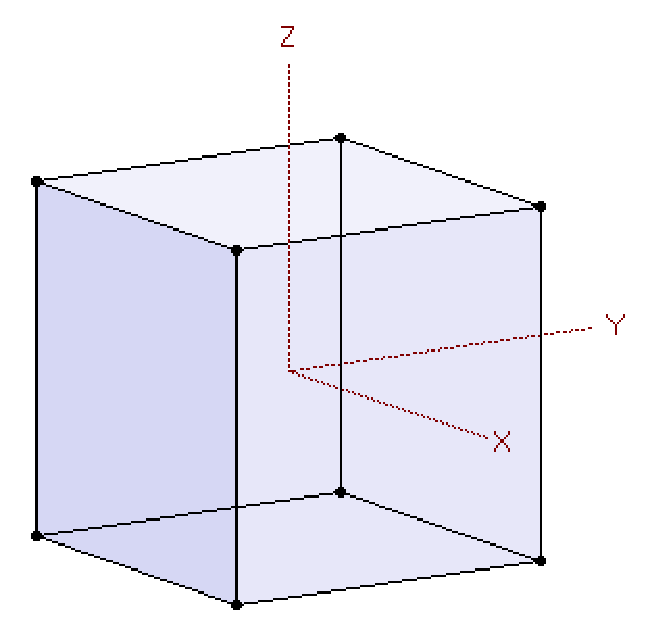
\includegraphics[width=2.5cm]{figures/cubic.pdf}       &
    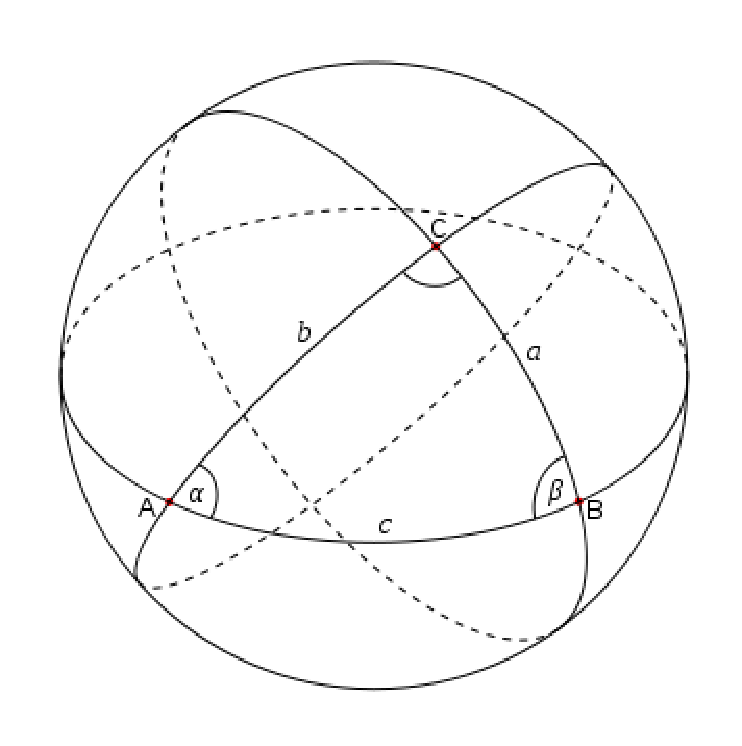
\includegraphics[width=2.5cm]{figures/spherical.pdf}   &
    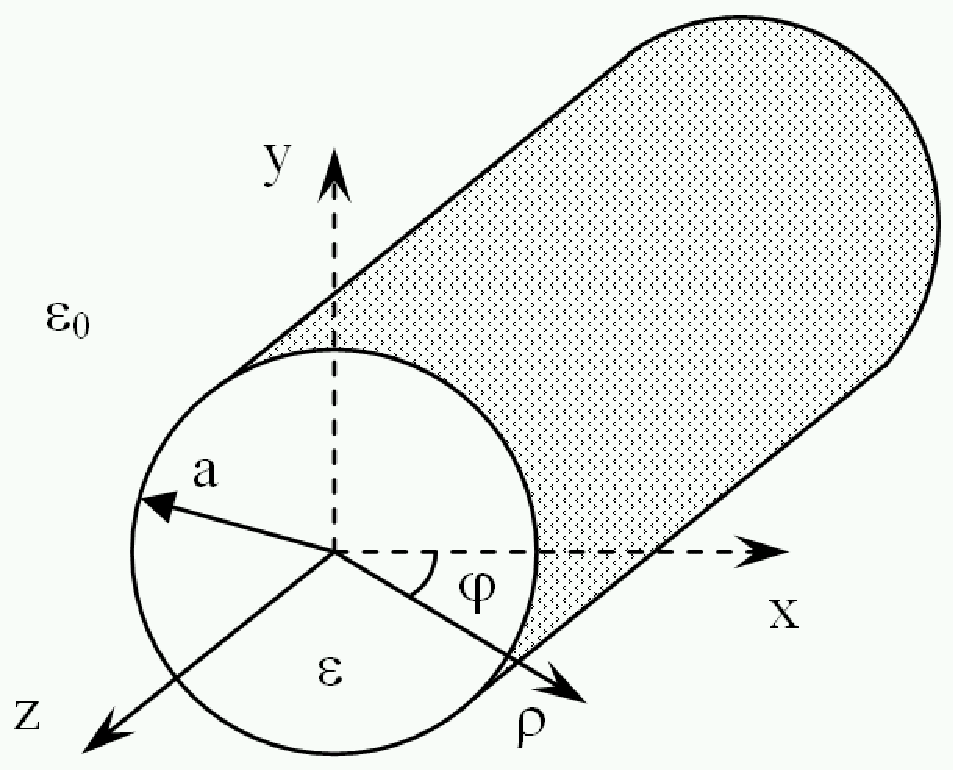
\includegraphics[width=2.5cm]{figures/cylindrical.pdf} 
    \\
    \\
    Spheroidal (prolate) & Spheroidal (oblate) & Ellipsoidal \\
    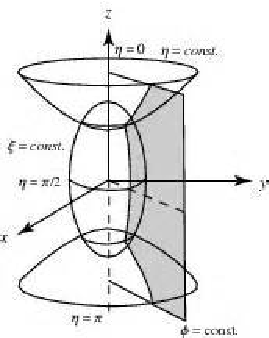
\includegraphics[width=2.5cm]{figures/prolate.pdf}     &
    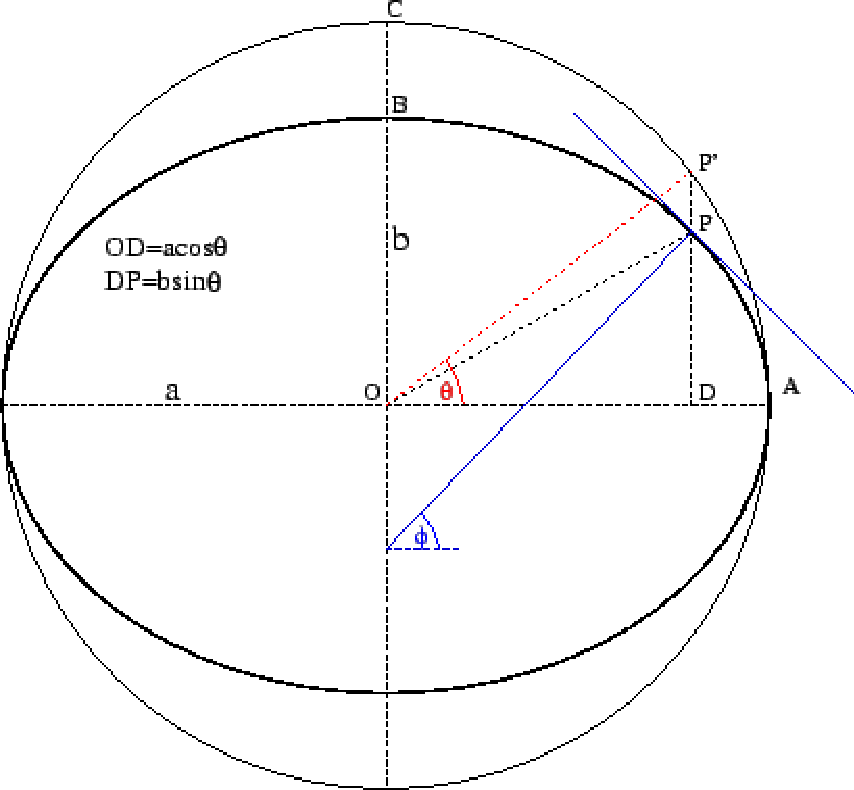
\includegraphics[width=2.5cm]{figures/oblate.pdf}      &
    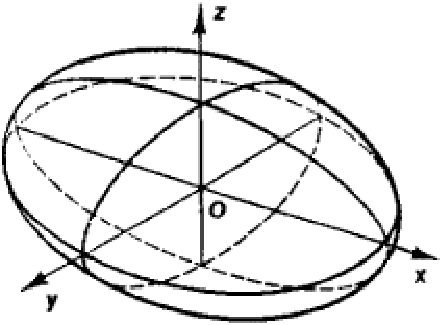
\includegraphics[width=3cm]{figures/ellipsoid.pdf}
\end{tabular}
}
\end{frame}


\subsection{Numerical}

\begin{frame}
\frametitle{Why Finite Elements?}

\begin{block}{Finite elements are flexible enough to handle}
\begin{itemize}
\item Any geometry
\item Inhomogeneous coefficients
\item Anisotropic tensors fields
\item Arbitrary boundary conditions
\end{itemize}
\end{block}

\vspace{2cm}
Lets see some examples ...
\end{frame}



\subsection{Industrial problems}

\begin{frame}
\frametitle{Aerodynamics}
  \begin{center}
   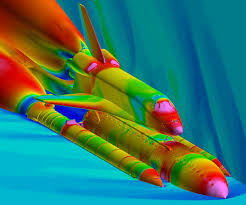
\includegraphics[width=0.45\textwidth]{figures/Apollo.jpg}
   \hfill
   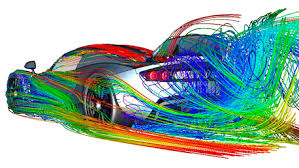
\includegraphics[width=0.45\textwidth]{figures/MacLaren.png}
   \vfill
   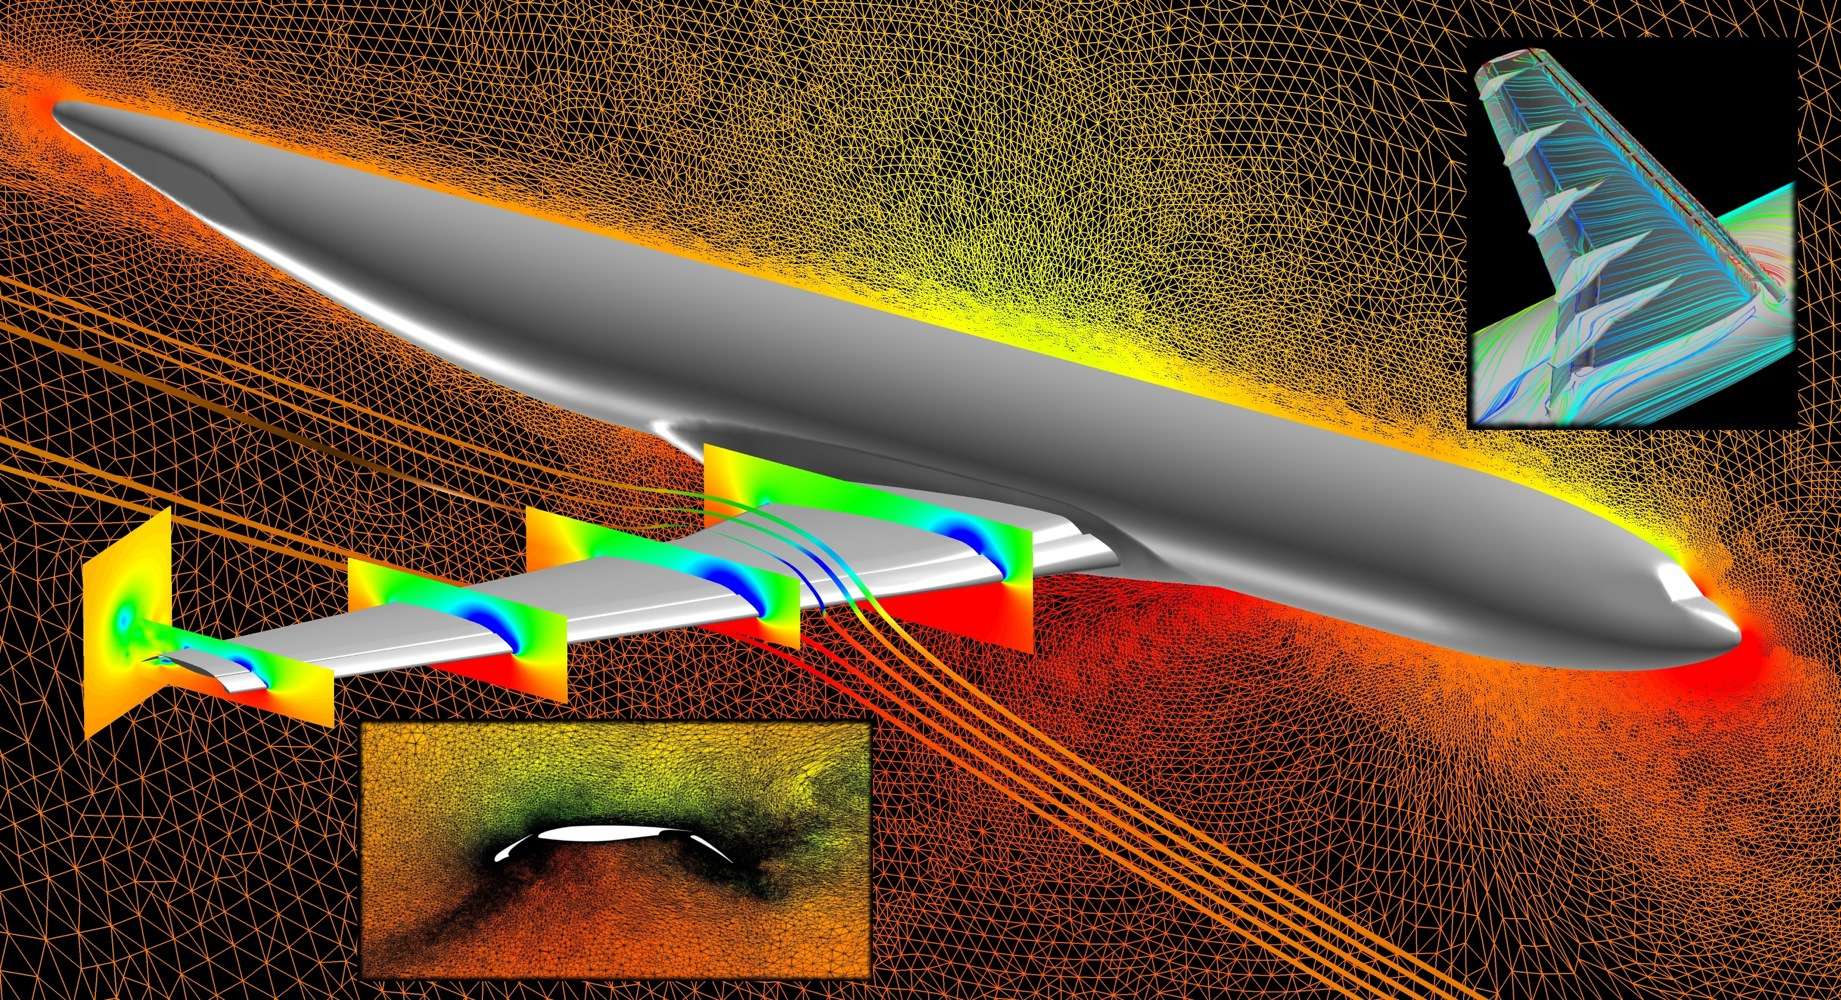
\includegraphics[width=0.45\textwidth]{figures/Nielsen.jpg}
   \hfill
  %\includegraphics[width=2cm]{figures/JaguarExahighres.png}
  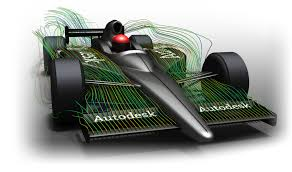
\includegraphics[width=0.45\textwidth]{figures/F1.jpg}
  \end{center}

\end{frame}



\begin{frame}
\frametitle{Structural Optimization}
  \begin{center}
   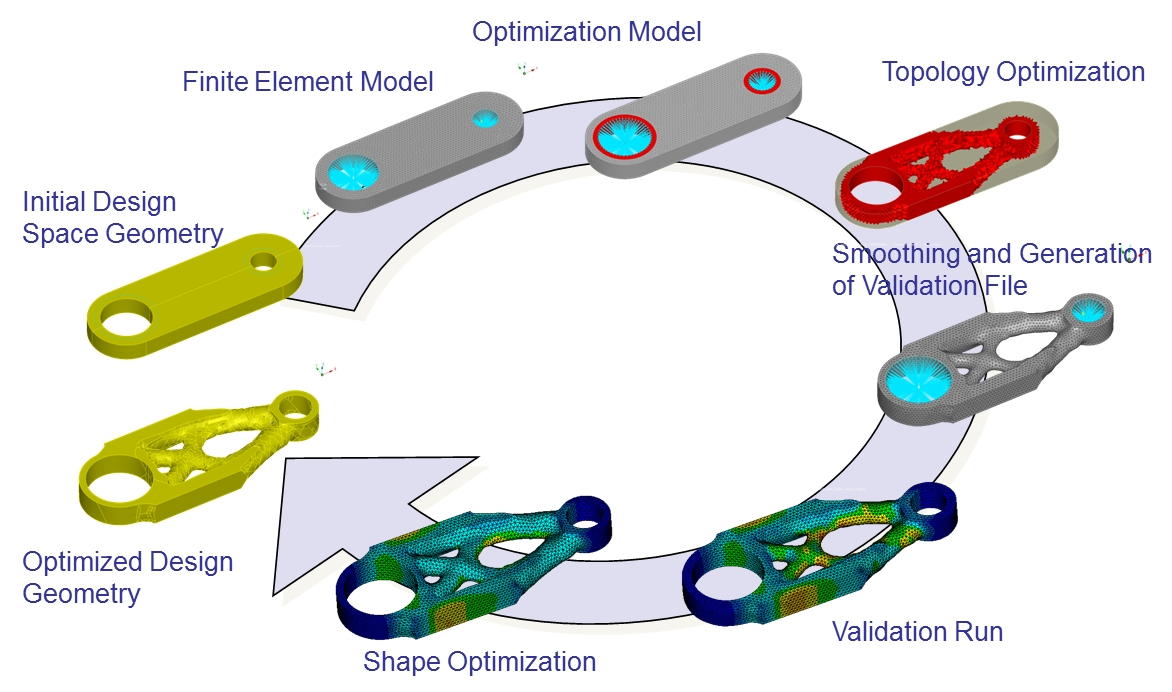
\includegraphics[width=0.6\textwidth]{figures/TOSCA.jpg}
   \vfill
  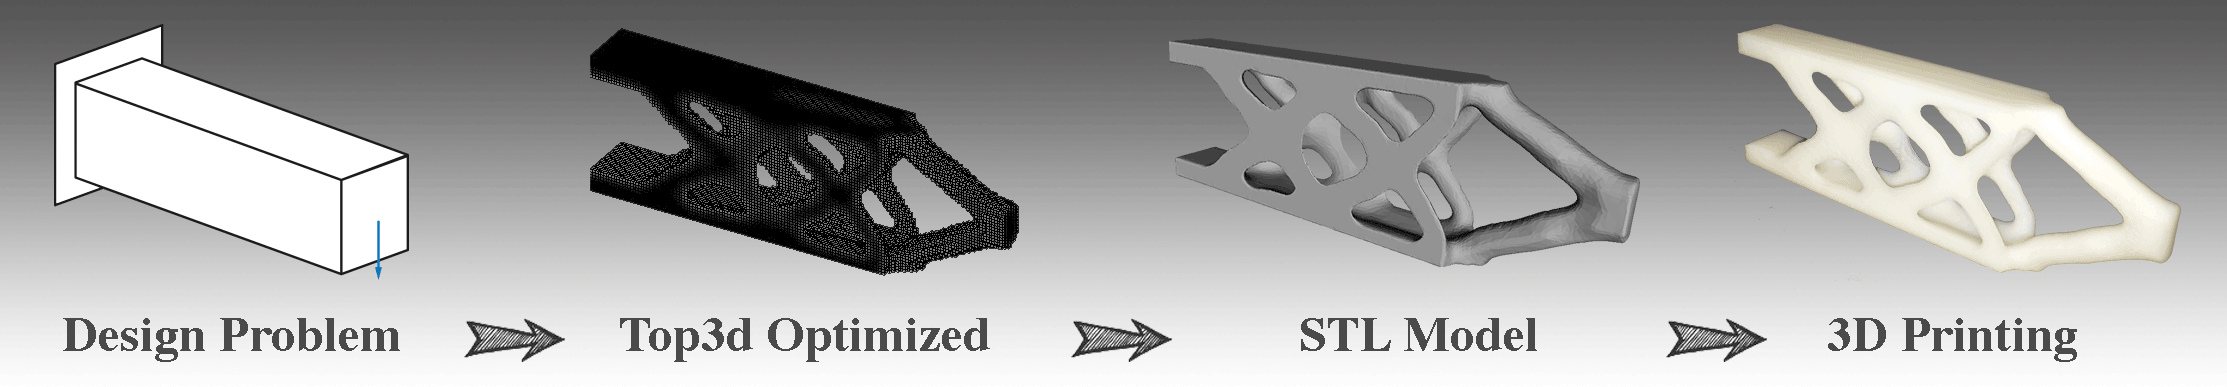
\includegraphics[width=0.85\textwidth]{figures/top3d_banner1.png}
  %\hfill
  % \includegraphics[width=0.5\textwidth]{figures/TourbineVisit.png}
  \end{center}

\end{frame}




\begin{frame}
\frametitle{Brain, heart: biomedical applications}
\begin{center}
\begin{tabular}{cc}
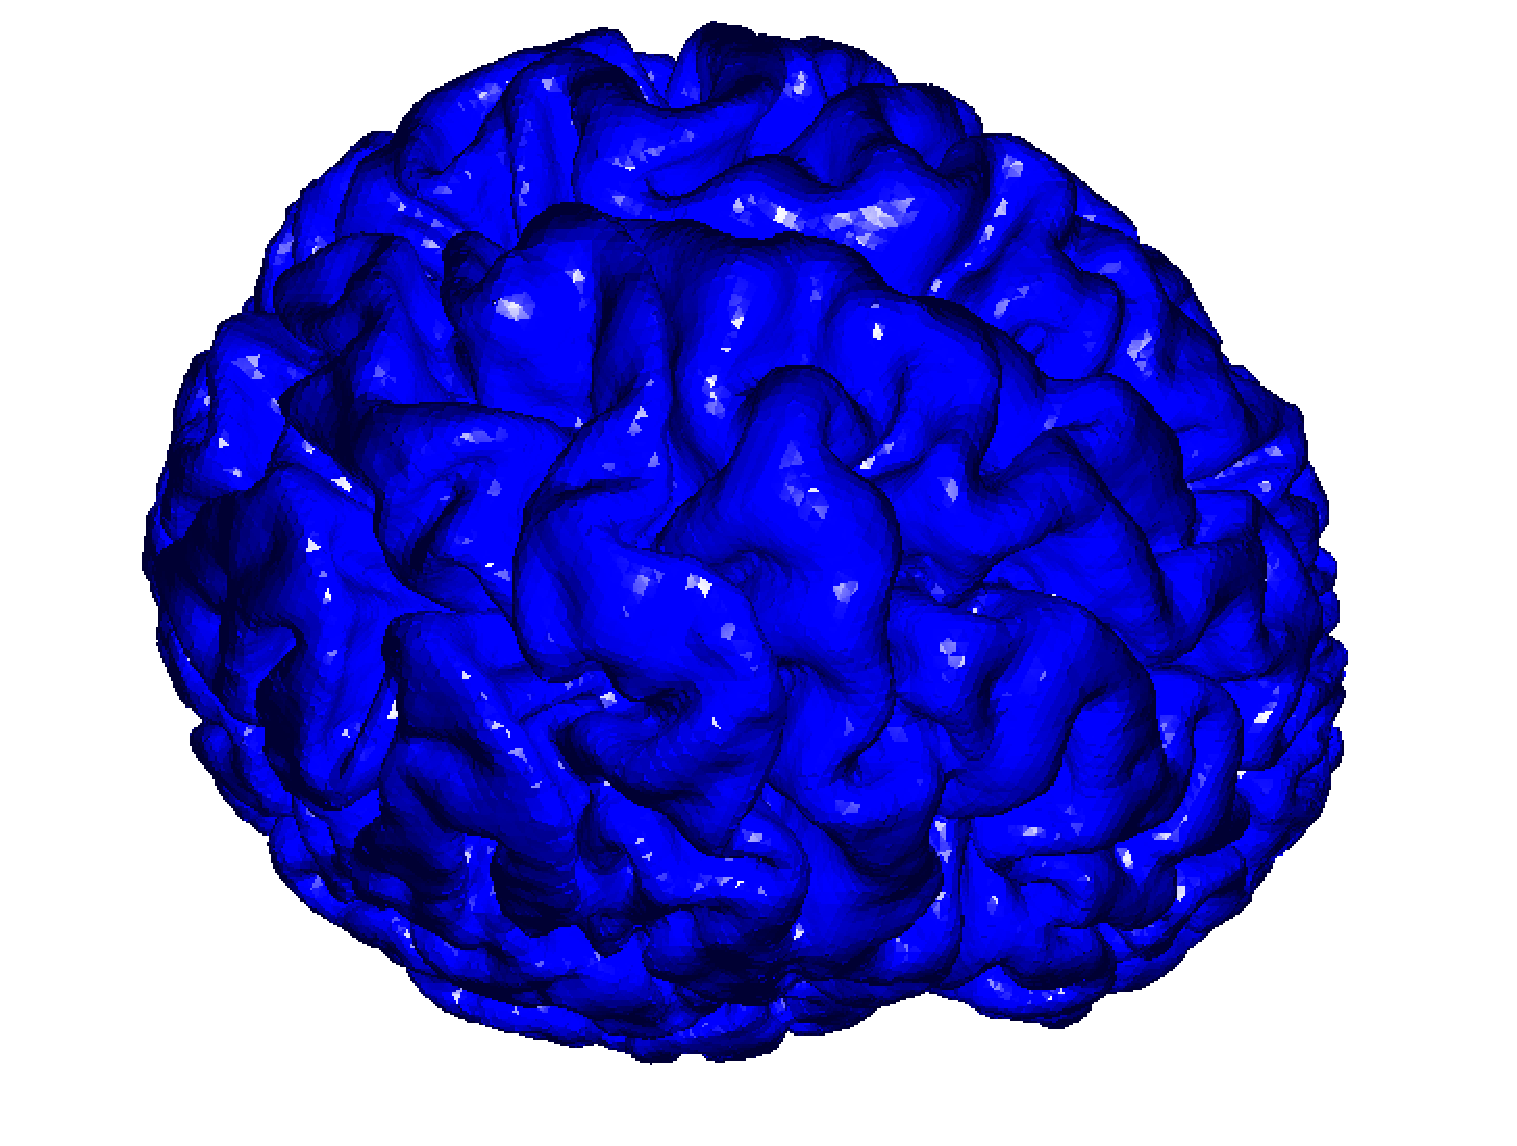
\includegraphics[totalheight=2in,angle=0]{figures/brain1.pdf} &
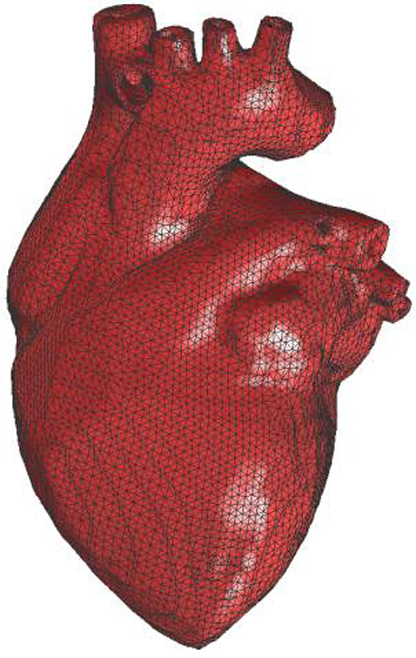
\includegraphics[totalheight=2in,angle=0]{figures/heart.jpg} \\
Source localization & Heart simulation
\end{tabular}
\end{center}
\end{frame}


\begin{frame}
\frametitle{Reservoir simulation}
  \begin{center}
   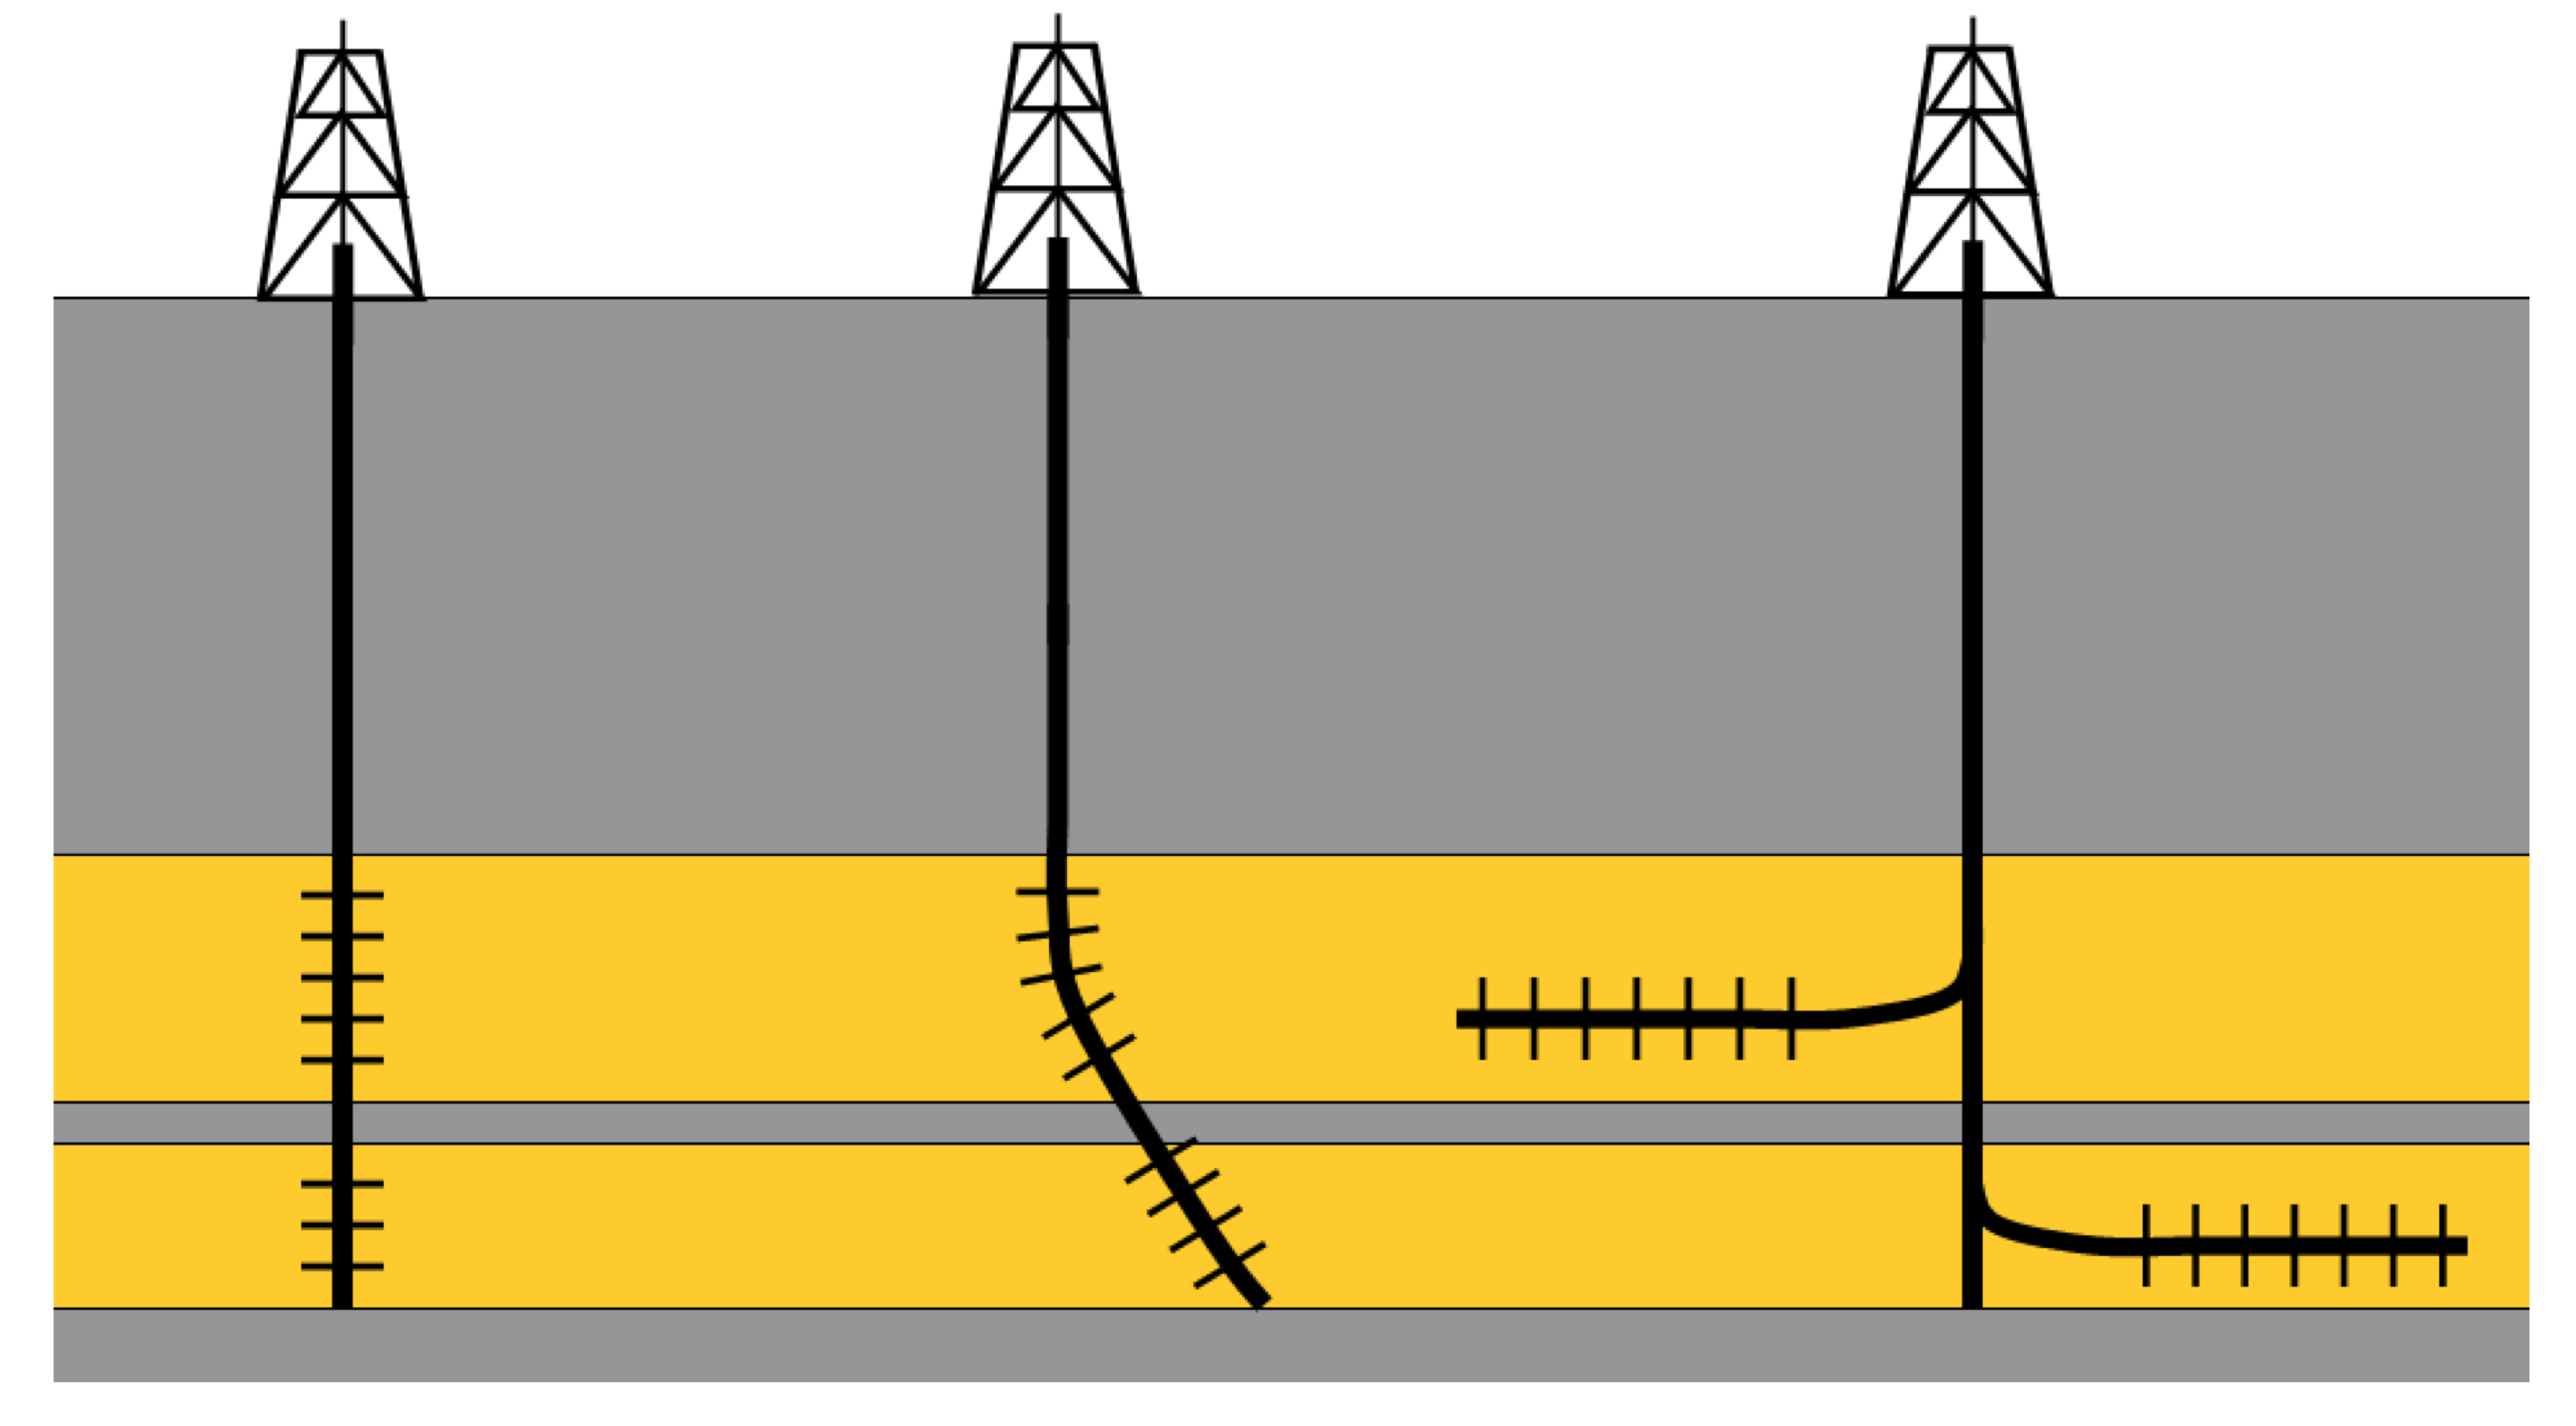
\includegraphics[width=5cm,height=4.cm]{figures/WellTypes.png}
   \hfill
   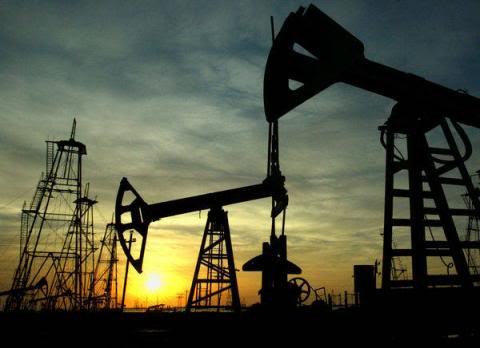
\includegraphics[height=4.cm]{figures/oil-field-tmr.jpg}
   \vfill
   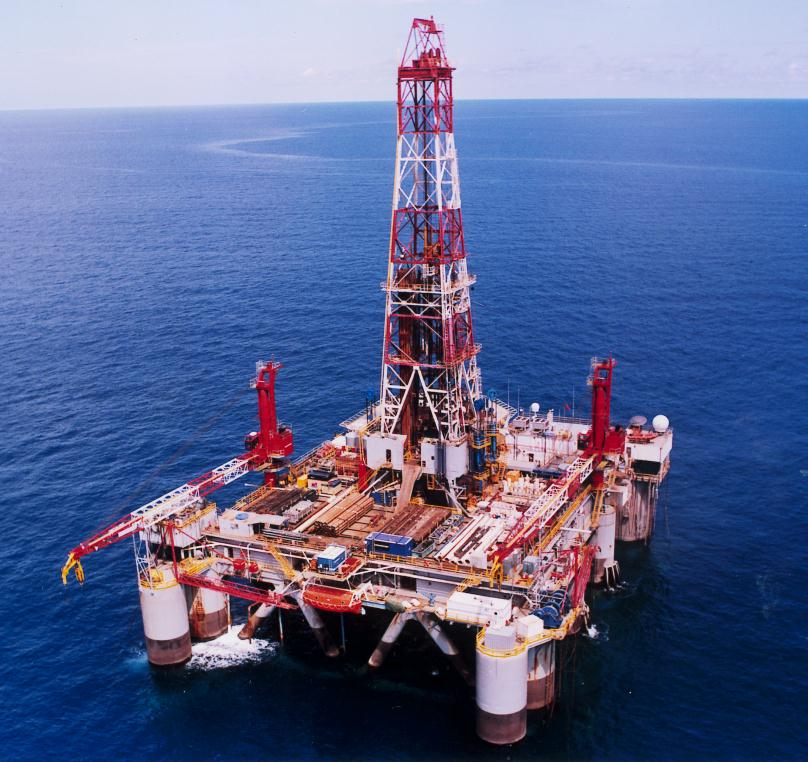
\includegraphics[width=5cm,height=3.5cm]{figures/Offshore.jpg}
   \hfill
   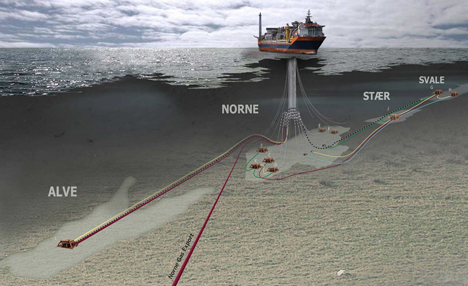
\includegraphics[height=3.4cm]{figures/Norne.png}
  \end{center}
\end{frame}

\begin{frame}
\frametitle{Reservoir simulation}

\begin{tabular}{cc}
Johansen formation & Norne field \\
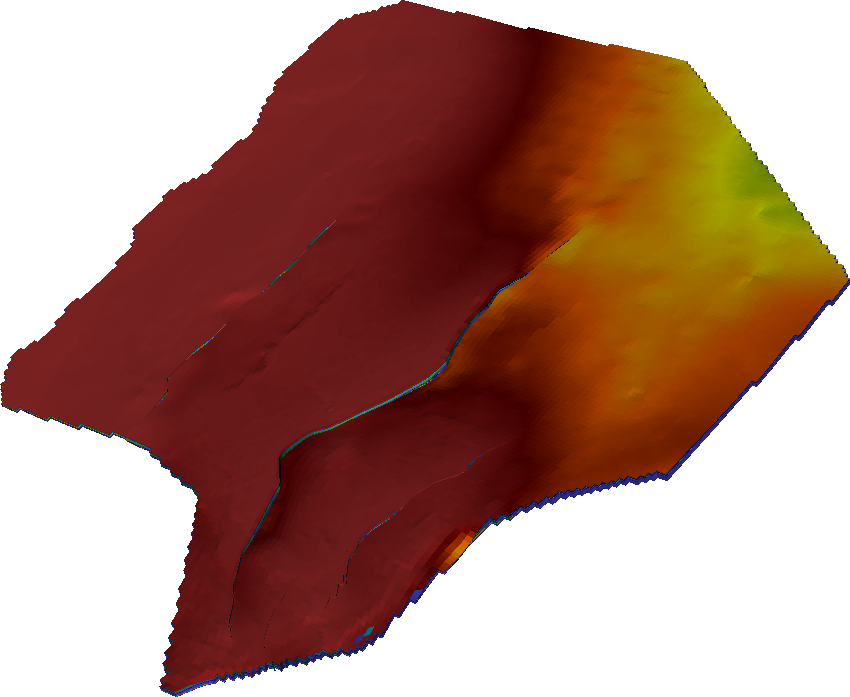
\includegraphics[totalheight=1.5in,angle=0]{figures/Johansen.png} &
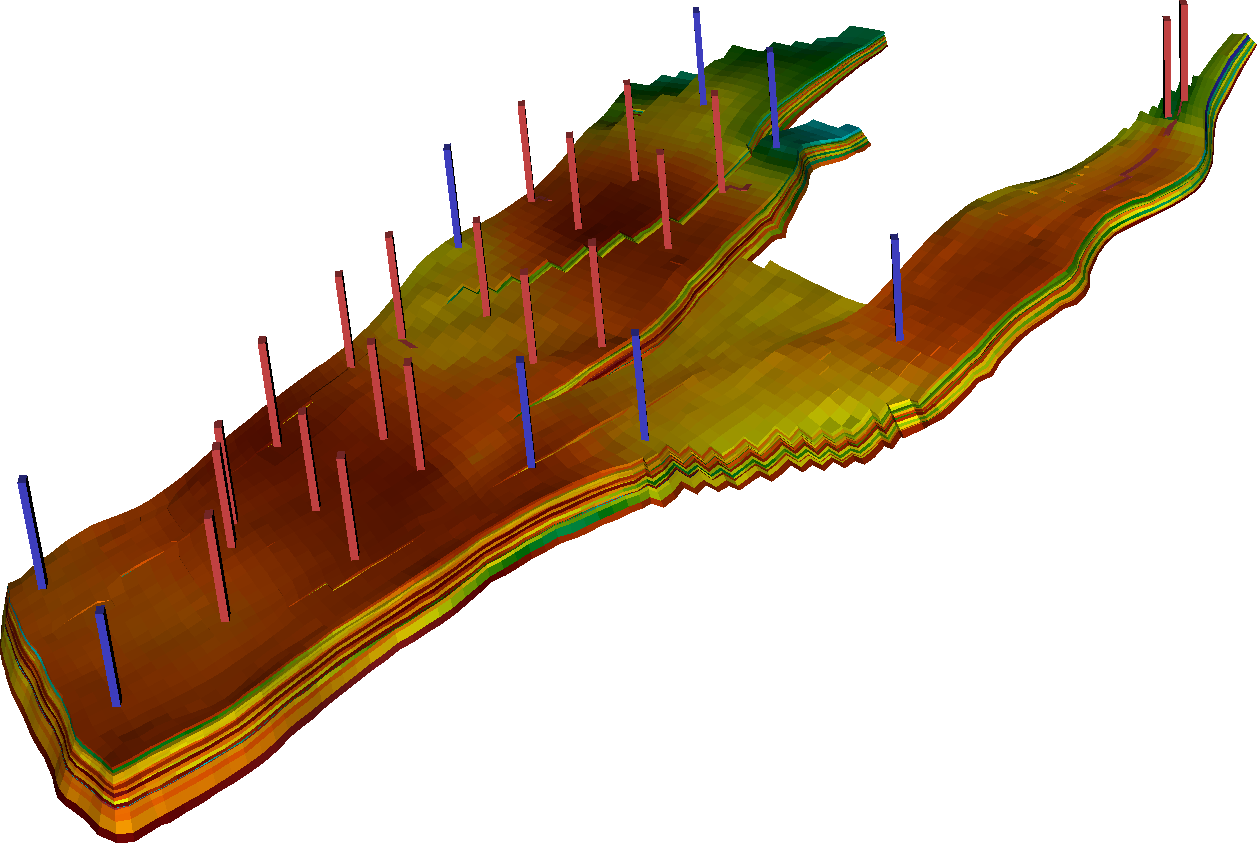
\includegraphics[totalheight=1.5in,angle=0]{figures/NorneModelPermeabilityMap}
\end{tabular}
\begin{center}
Inhomogeneous and anisotropic tensor fields (permeability)
\end{center}
\end{frame}


\begin{frame}
\frametitle{Seismic Inversion}
  \begin{center}
   \begin{minipage}{0.45\textwidth}
   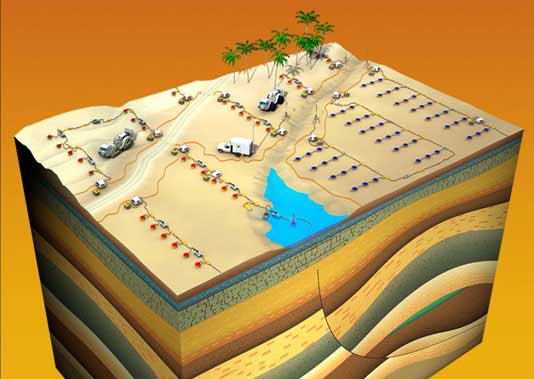
\includegraphics[width=\textwidth]{figures/scorpion_landscape.jpg}
   \end{minipage}
   \hfill
   \begin{minipage}{0.45\textwidth}
   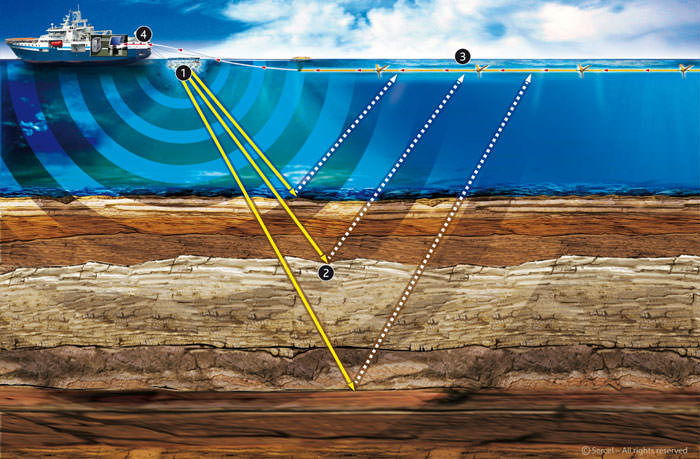
\includegraphics[height=0.7\textwidth, width=\textwidth]{figures/MarineSeismic.jpg}
   \end{minipage}
   \vfill
   \begin{minipage}{0.45\textwidth}
   \scriptsize{
   \begin{block}{Acoustic, Elastic waves}
   \begin{itemize}
   \item[] $$\rho \pder{^2 \u}{t^2} - \nabla \cdot \boldsymbol{\sigma} = \rho \f $$
   \end{itemize} 
   \end{block}}
   \end{minipage}
   %\begin{minipage}{0.4\textwidth}
   %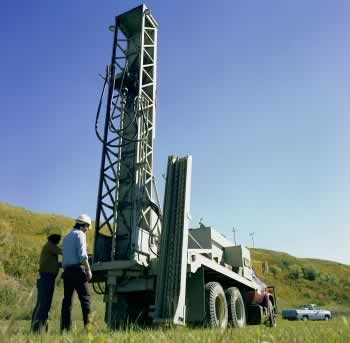
\includegraphics[width=\textwidth]{figures/seismic__land350.jpg}
   %\end{minipage}
   \hfill
   \begin{minipage}{0.45\textwidth}
   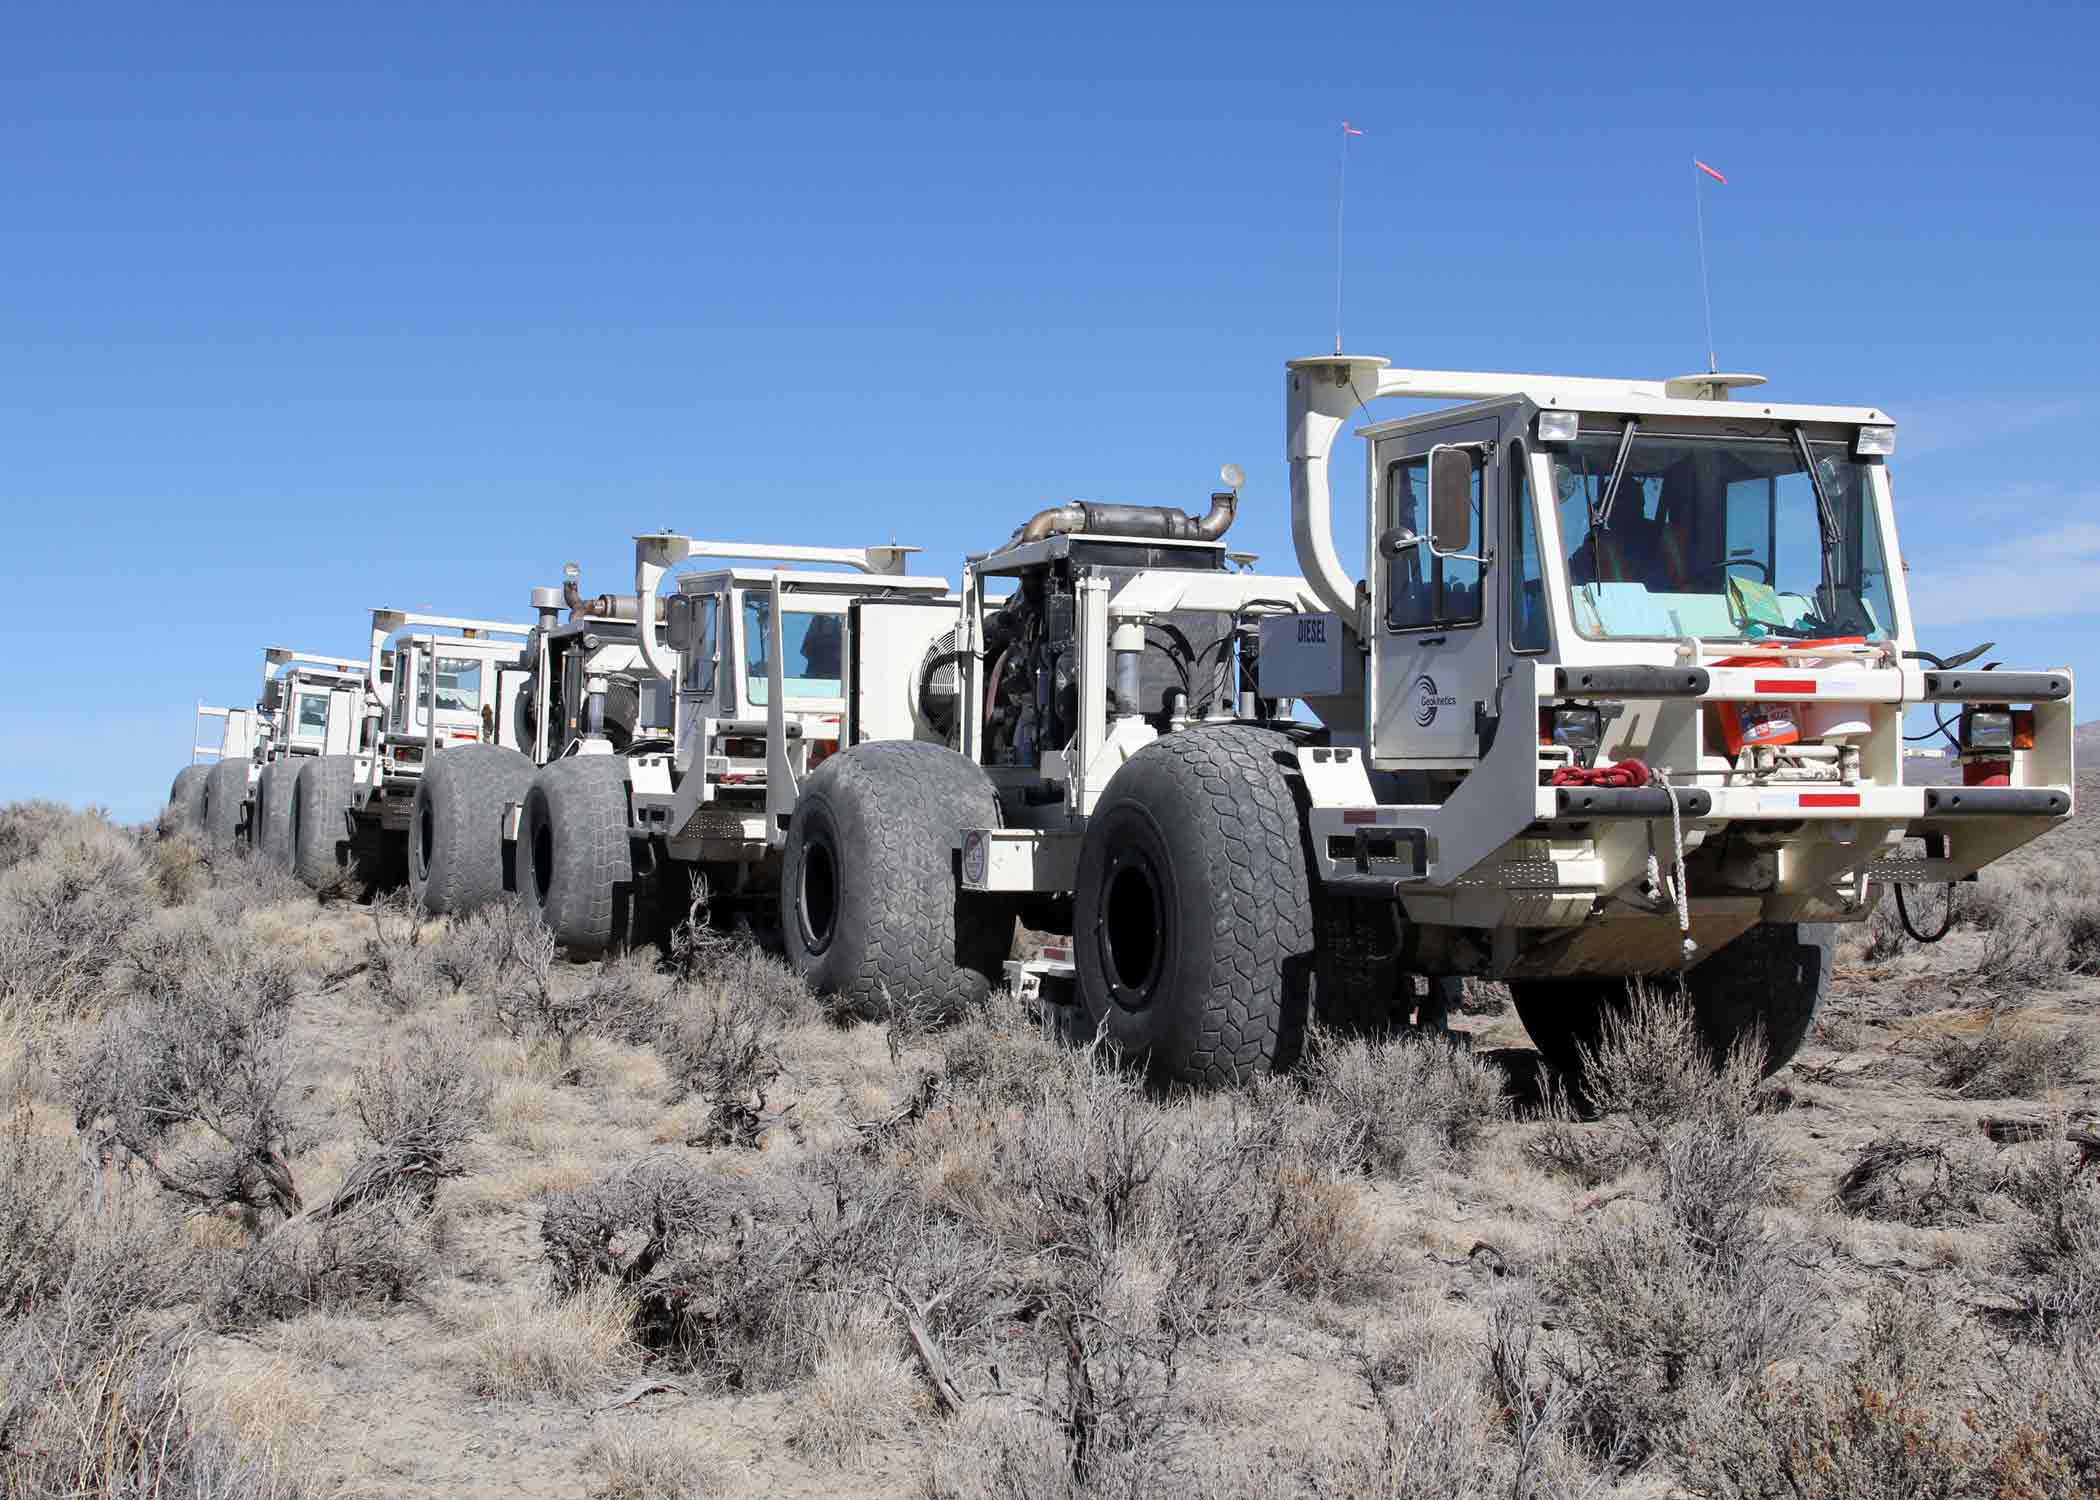
\includegraphics[height=0.6\textwidth,width=\textwidth]{figures/trucks.jpg}
   \end{minipage}
  
  \end{center}
\end{frame}



\section{Mesh generation}


\begin{frame}{Grid Systems}
\centering
\begin{tabular}{cc}
Block-centered grid & Point-distributed grid \\
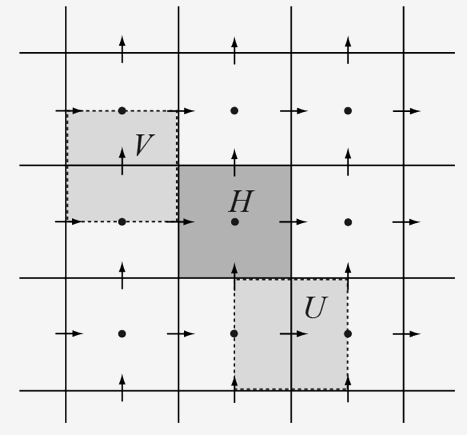
\includegraphics[width=0.35\textwidth]{figures/cellQuad.png}
&
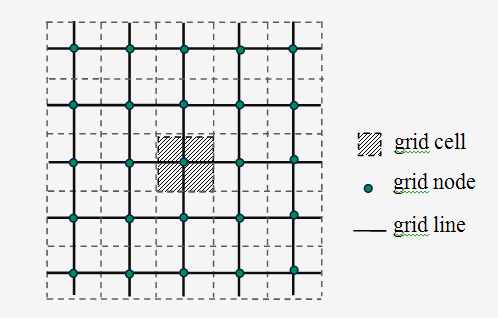
\includegraphics[width=0.51\textwidth]{figures/pointQuad.png}
\end{tabular}
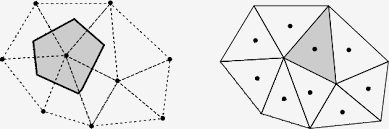
\includegraphics[width=0.5\textwidth]{figures/cellcentered.png}
\end{frame}




\begin{frame}{Grids}
\begin{tabular}{cc}
PEBI          & Voronoi cells \\
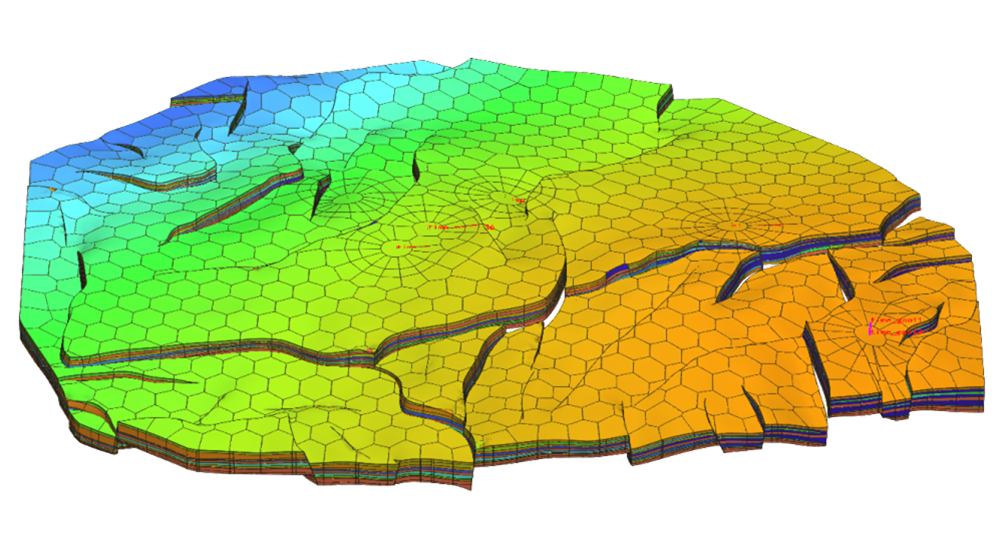
\includegraphics[width=0.45\textwidth]{figures/PEBI1.png}
&
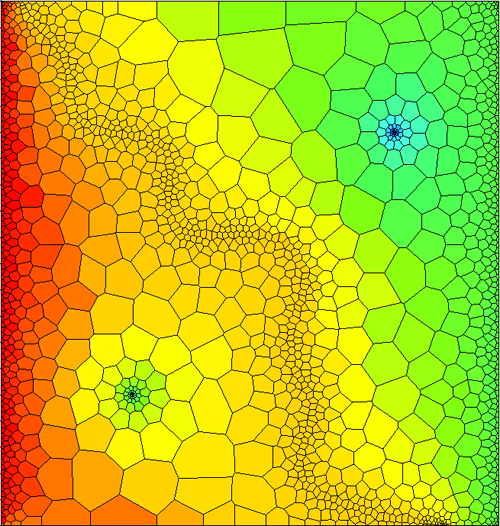
\includegraphics[width=0.25\textwidth]{figures/voronoi-cells2D.png} \\
Corner point &      \\
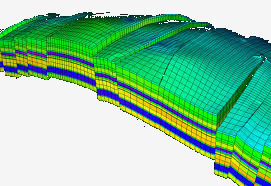
\includegraphics[width=0.45\textwidth]{figures/CPGgridm.png}
&
%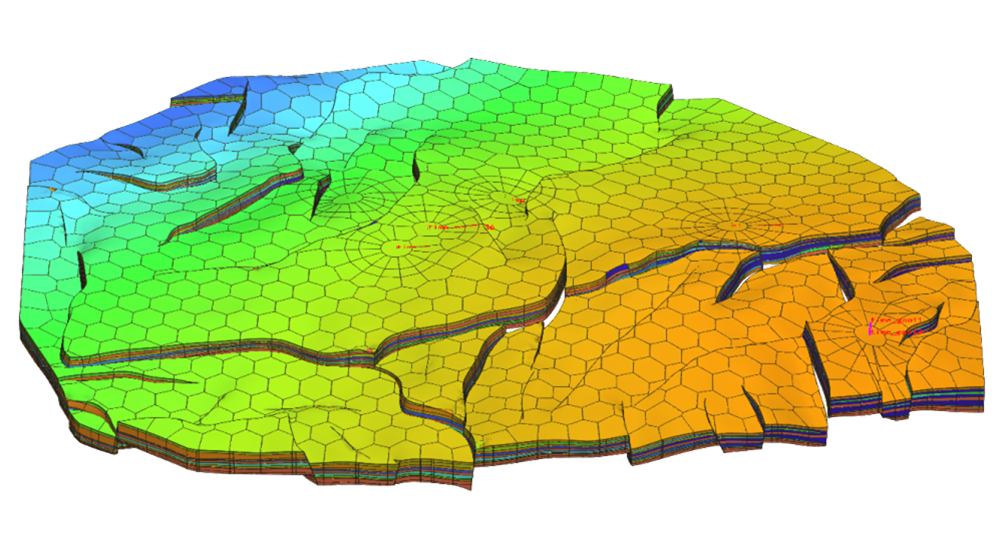
\includegraphics[width=0.45\textwidth]{figures/PEBI1.png}
\end{tabular}
\end{frame}

\begin{frame}
\frametitle{The 3D case can be very challenging}
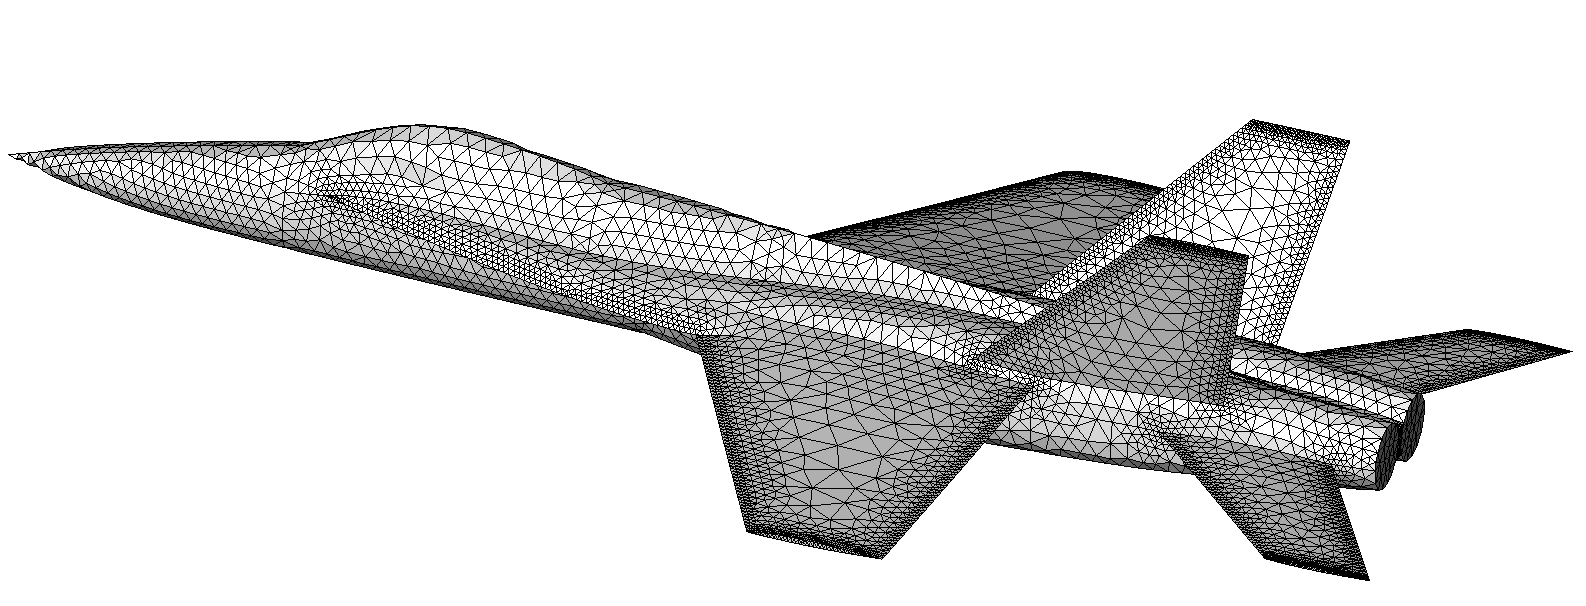
\includegraphics[width=\textwidth]{figures/F17.png}
\end{frame}



\section{Discretization}


\begin{frame}
\frametitle{2D and 3D Finite Elements}
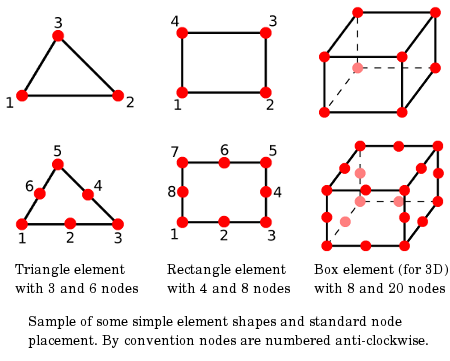
\includegraphics[width=0.8\textwidth]{figures/FiniteElements.png}
\end{frame}



\section{Linear Algebra}
\subsection{The linear system}
% @@@@@@@@@@@@@@@@@@@@@@@@@@@@@@@@@@@@@@@@@@@@@@@@@@@@@@@@@@@@@@@@@@@@@@
% @                                                                    @
% @ PROBLEMS IN 2D                                                     @
% @                                                                    @
% @@@@@@@@@@@@@@@@@@@@@@@@@@@@@@@@@@@@@@@@@@@@@@@@@@@@@@@@@@@@@@@@@@@@@@

\begin{frame}{The linear system}
\begin{block}{After discretization in space or space and time we end up with}
\begin{align*}
           A\: x &= b, \quad \text{or in the time dependent case}, \\
           A_n\: x_n &= b_n
\end{align*}
\end{block}

\begin{block}{Solution techniques}
\begin{itemize}
\item Direct sparse methods
\item Iterative methods
\end{itemize}
\end{block}
\end{frame}


\subsection{Direct sparse methods}

\begin{frame}{Direct sparse solvers}

\begin{center}

\begin{minipage}{0.45\textwidth}
\begin{block}{Complexity in 2D}
  \begin{itemize}
  \item O($N^{1.5}$) factorization 
  \item O($N \log N$) solution
  \end{itemize}  
\end{block}
\end{minipage}
\hfill
\begin{minipage}{0.45\textwidth}
\begin{block}{Complexity in 3D}
  \begin{itemize}
  \item \red{O($N^{2}$) factorization}
  \item O($N^{1.5}$) solution
  \end{itemize}  
\end{block}
\end{minipage}

\bigskip

\bigskip

\begin{minipage}{0.6\textwidth}
Available Software
{\small
  \begin{itemize}
  \item \blue{PARDISO}
  \item UMFPACK, CHOLMOD
  \item SUPERLU
  \item MUMPS
  \end{itemize}  
}
\end{minipage}

\end{center}

\end{frame}


\begin{frame}
\frametitle{Direct Sparse Solvers}
\begin{block}{PARDISO performance in 2D}
\begin{table}
\centering
\begin{tabular}{||r||r|r|r|r||r||}
  \hline
  \multicolumn{1}{||c||}{mesh}
      & \multicolumn{4}{c||}{Elapsed time in seconds}
      & \multicolumn{1}{c||}{memory} \\
  \hline
  nodes & init & fact & back-sub & total & MB~~~\\
  \hline
%     4014& 0.037 & 0.011 & \blue{0.001~} & 0.049 & \red{  1.4~~} \\
%    16454& 0.158 & 0.052 & \blue{0.004~} & 0.216 & \red{  5.9~~} \\
    65175& 0.704 & 0.265 & \blue{0.019~} & 0.988 & \red{ 26.0~~} \\
   263838& 3.199 & 1.539 & \blue{0.111~} & 4.849 & \red{117.5~~} \\
  1068112& 14.766& 9.518 & \blue{0.535~} &24.819 & \red{527.7~~} \\
  \hline
\end{tabular}
\end{table}
\end{block}

\begin{block}{PARDISO performance in 3D}
\begin{table}
\centering
\begin{tabular}{||r||r|r|r|r||r||}
  \hline
  \multicolumn{1}{||c||}{mesh}
      & \multicolumn{4}{c||}{Elapsed time in seconds}
      & \multicolumn{1}{c||}{memory} \\
  \hline
  nodes   & init & fact & back-sub & total & MB~~~ \\
  \hline
%      500 &  0.005 &    0.001 & \blue{0~}     & 0.006 & \red{    0.3~} \\ 
%     4001 &  0.062 &    0.057 & \blue{0.002~} & 0.121 & \red{    4.7~} \\
    32002 &  0.636 &    2.783 & \blue{0.069~} & 3.488 & \red{   80.4~} \\
   256011 &  6.925 &  185.469 & \blue{1.428~} & 193.8 & \red{ 1438.3~} \\
  2000396 & 76.625 & 11762.1  & \blue{21.46~} & 11860 & \red{24403.0~}  \\
  \hline
\end{tabular}
\end{table}
\end{block}


\end{frame}


\subsection{Iterative methods}

\begin{frame}
\frametitle{Iterative Krylov subspace methods}

They work with matrix-vector products $Ay$ for given vectors $y$
\begin{columns}[t]
\column{.45\textwidth}
\begin{block}{Symmetric systems}
\begin{itemize}
\item \blue{\bf{PCG}}
\item \blue{\bf{MINRES}}
\item \blue{\bf{SYMMLQ}}
\item \blue{\bf{LSMR}}
\item \blue{\bf{SQMR}}
\end{itemize}
\end{block}

\column{.45\textwidth}
\begin{block}{Nonsymmetric systems}
\begin{itemize}
\item \red{\bf{GMRES}}
\item \red{\bf{CGS}}
\item \red{\bf{BICGSTAB}}
\item \red{\bf{QMR}}
\item \red{\bf{LSQR}}
\end{itemize}
\end{block}
\end{columns}


\end{frame}




\begin{frame}{Generalized minimum residual methods}
\centering
\footnotesize{
\begin{minipage}{0.48\linewidth}
\begin{block}{\footnotesize {\textcolor{blue}{GMRES}(A,M,b,tol)}}
\vspace{-0.5cm}
\begin{align*}
   &x_0 = M^{-1}b, \; r_0 = b - Ax_0, \\ 
   &\beta = \Vert r_0 \Vert_2 \; u_1 = \frac{r_0}{\beta}, \; k = 0 \\
   &\text{while} \quad \Vert r_k \Vert_2 > \beta \; tol  \\
   &\quad k = k + 1 \; \blue{z_k = M^{-1} v_k, \; w = Az_k} \\
   &\quad \text{for} \; i = 1,2,\ldots,k \; \text{do} \\
   &\quad \quad h_{i,k} = u_i^T w, \; w = w - h_{i,k} u_i \\
   &\quad \text{end for} \\
   &\quad h_{k+1,k} = \Vert w \Vert_2, \; u_{k+1} = \frac{w}{h_{k+1,k}} \\
   &\quad V_k = [v_1, \ldots, v_k] \\ 
   &\quad H_k = \{h_{i,j}\}, \; 1\le i \le j+1, \; 1 \le j \le k \\
   &\quad y_k = \text{argmin}_y \Vert \beta e_1 - H_k \:  y \Vert_2 \\
   &\quad \textcolor{blue}{x_k = x_0 + M^{-1} V_k \: y_k}, \; r_k = b-A \: x_k \\
   &\text{end while}
\end{align*}
\end{block}
\end{minipage}
\hfill
\begin{minipage}{0.48\linewidth}
\begin{block}{\footnotesize {\textcolor{red}{FGMRES}(A,M,b,tol)}}
\vspace{-0.5cm}
\begin{align*}
   &x_0 = M^{-1}_0b, \; r_0 = b - Ax_0, \\ 
   &\beta = \Vert r_0 \Vert_2 \; u_1 = \frac{r_0}{\beta}, \; k = 0 \\
   &\text{while} \quad \Vert r_k \Vert_2 > \beta \; tol  \\
   &\quad k = k + 1, z_k = M^{-1}_k v_k, \; w = Az_k \\
   &\quad \text{for} \; i = 1,2,\ldots,k \; \text{do} \\
   &\quad \quad h_{i,k} = u_i^T w, \; w = w - h_{i,k} u_i \\
   &\quad \text{end for} \\
   &\quad h_{k+1,k} = \Vert w \Vert_2, \; u_{k+1} = \frac{w}{h_{k+1,k}} \\
   &\quad V_k = [v_1, \ldots, v_k], \; \textcolor{red}{Z_k = [z_1, \ldots, z_k]} \\ 
   &\quad H_k = \{h_{i,j}\}, \; 1\le i \le j+1, \; 1 \le j \le k \\
   &\quad y_k = \text{argmin}_y \Vert \beta e_1 - H_k \:  y \Vert_2 \\
   &\quad \textcolor{red}{x_k = x_0 + Z_k \: y_k}, \; r_k = b-A \: x_k \\
   &\text{end while}
\end{align*}
\end{block}
\end{minipage}
}
\end{frame}



\begin{frame}
\frametitle{Sophisticated iterative methods: domain decomposition}

\begin{center}
  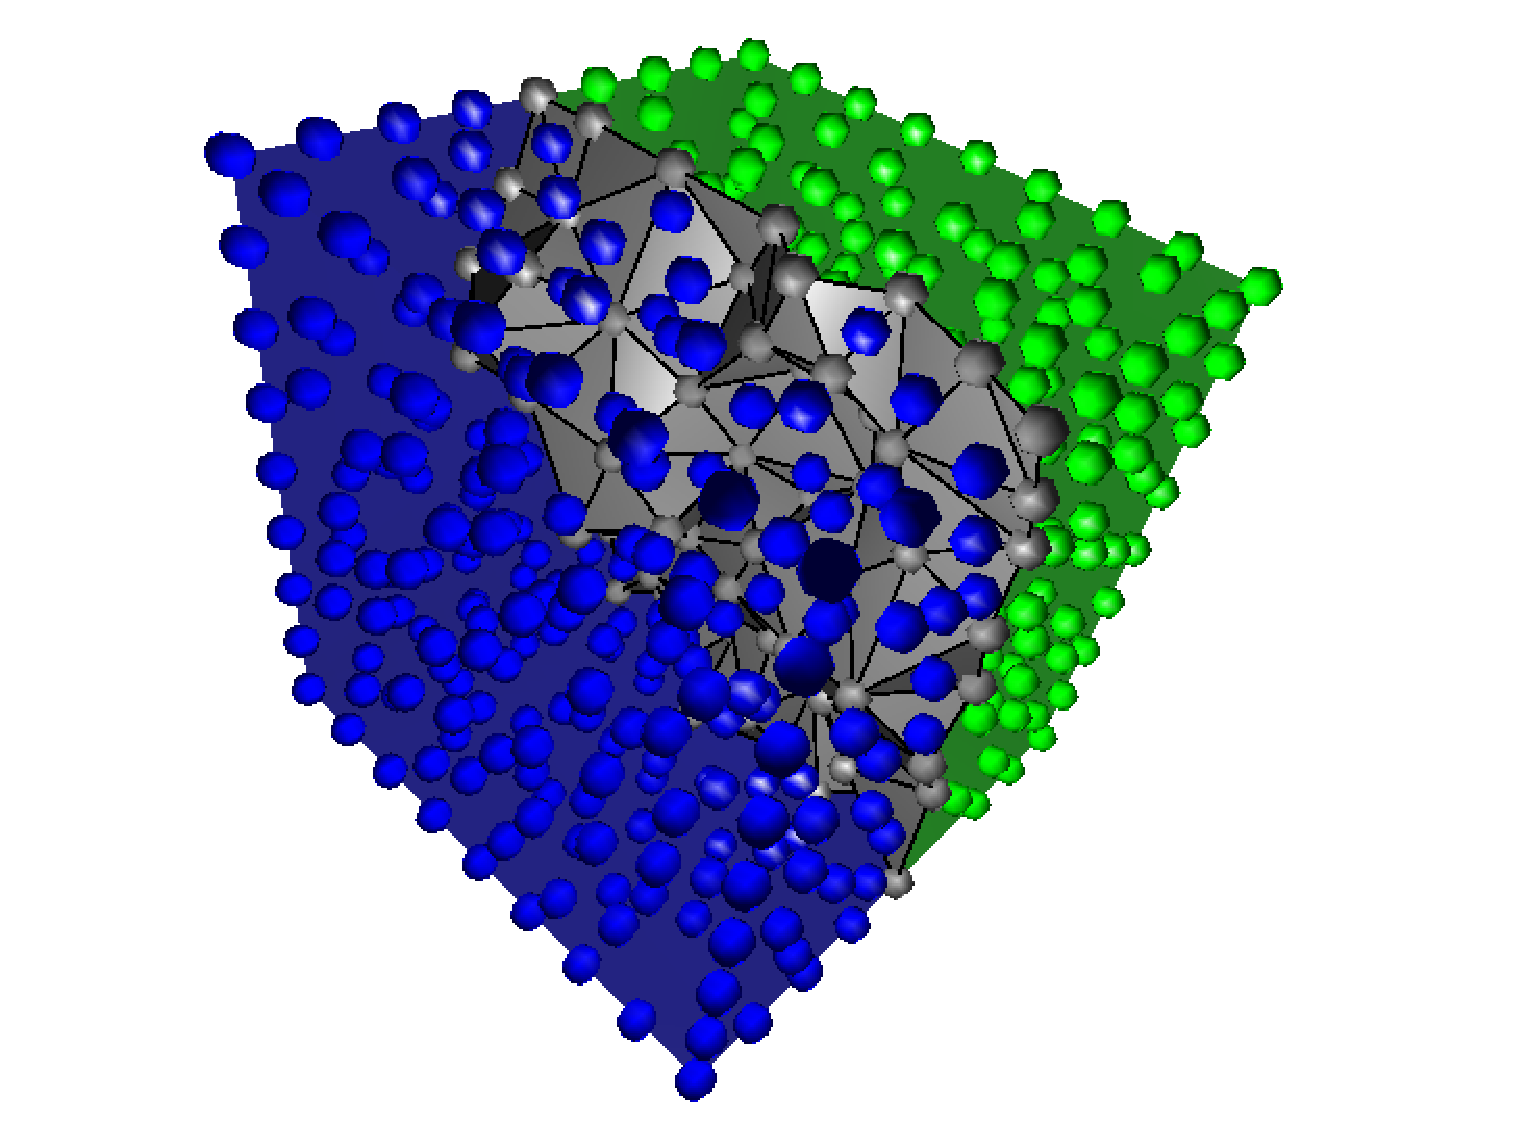
\includegraphics[width=6.0cm]{figures/3Ddomain-2parts.pdf}
  \hspace*{-1.0cm}
  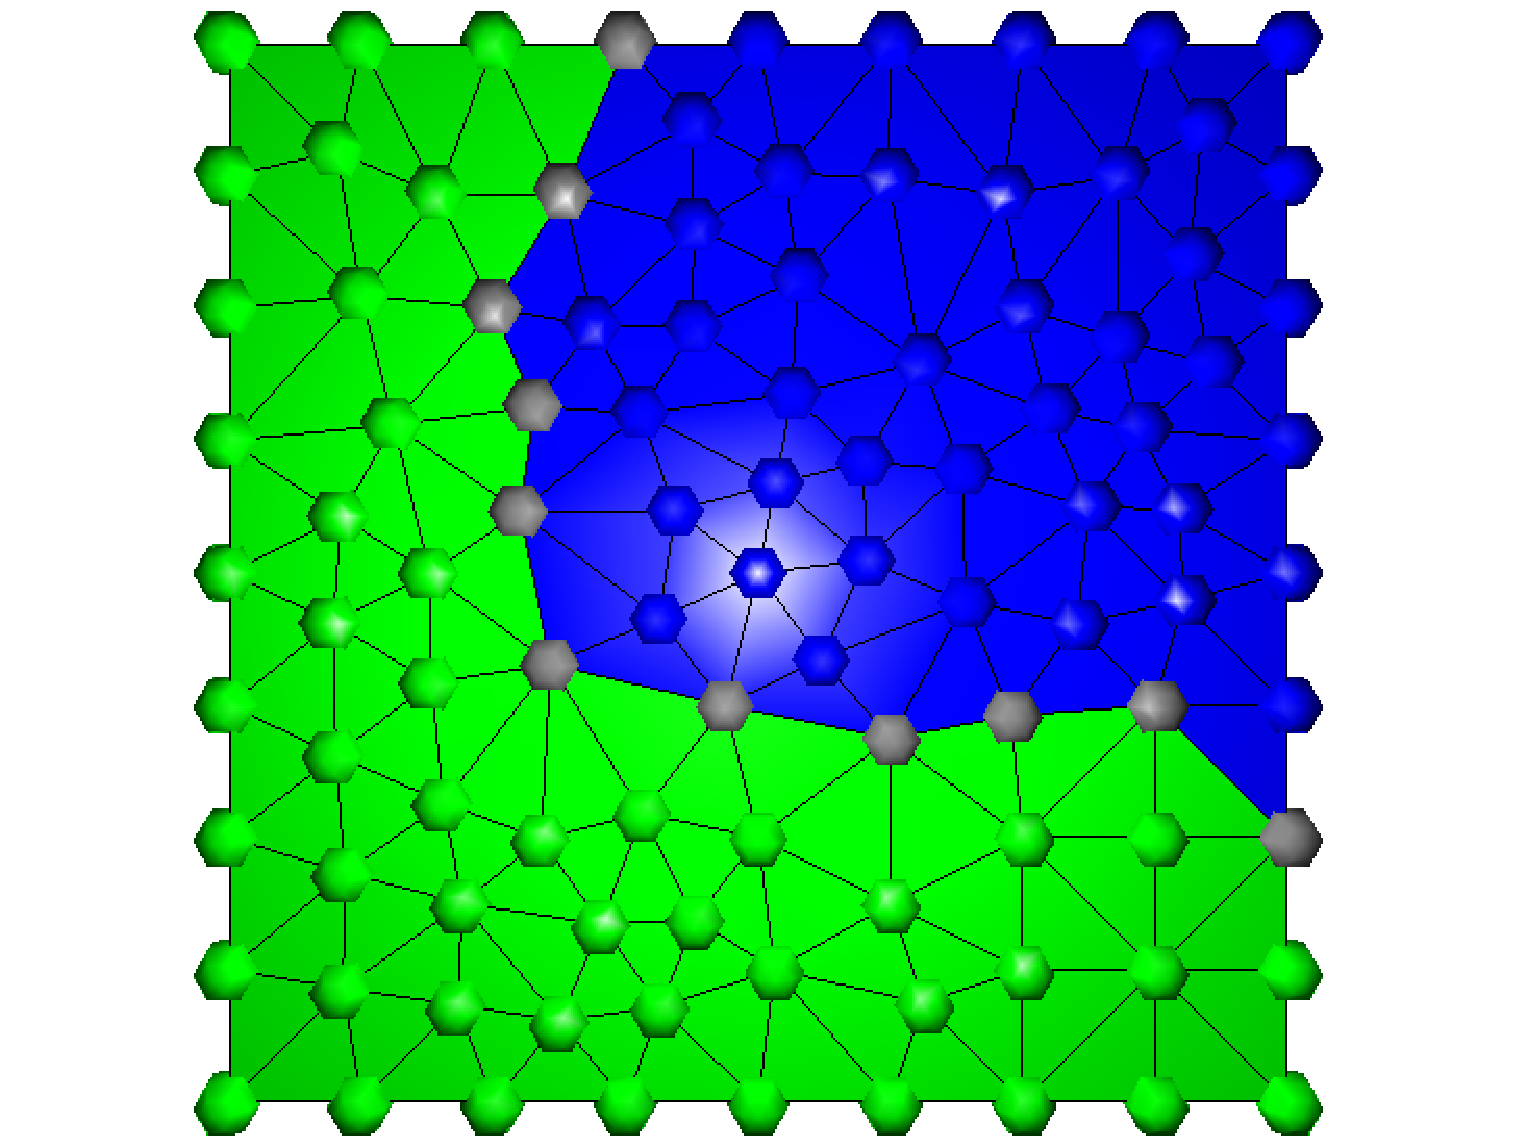
\includegraphics[width=6.0cm]{figures/2subdomain.pdf}
\end{center}
\Large{
\[
\pmat
{
  \green{A_{11}}    & 0         & \green{A_{1B}} \\
  0         & \blue{A_{22}}     & \blue{A_{2B}}  \\
  \gray{A_{1B}^T}  & \gray{A_{2B}^T}  & \gray{A_{BB}}
}
\,
\pmat
{
  \green{u_1} \\
  \blue{u_2}  \\
  \gray{u_B}
}
=
\pmat
{
  \green{f_1} \\
  \blue{f_2}  \\
  \gray{f_B}
}
\]}
%Internal boundary Schur complement
%$$S_B=A_{BB}-A_{1B}^TA_{11}^{-1}A_{1B}-A_{2B}^TA_{22}^{-2}A_{2B}$$
%$S_B$ is the discretization of the Steklov-Poincar\'{e} operator ${\cal S}$
\end{frame}


\begin{frame}
\frametitle{Our journey to the Finite Element realm}

\begin{block}{will step through}
\begin{enumerate}
\item {\it the} {\bf Mesh generation} (IO)\footnote{\url{https://wci.llnl.gov/simulation/computer-codes/visit/}}   
\item {\it the} {\bf Discretization}  (Hexahedra/Tetrahedra)
\item {\it the} {\bf Linear Algebra}  (Direct/Iterative solvers)
\item {\it the} {\bf Sparse Linear Algebra}
\item {\it the} {\bf Implementation} in {\small MATLAB}\footnote{\url{http://www.mathworks.ch/moler/exm/book.pdf}}
\item {\it the} {\bf Assignments} in \hologo{LaTeX}\footnote{\url{https://www.macports.org} \fbox{\$sudo port install texlive +full}}
\item {\it the} {\bf Additional Software} in \small{FEnICS}\footnote{\url{http://fenicsproject.org}}
\end{enumerate}
\end{block}

\end{frame}


\tikzset{redstyle/.style={circle,draw,fill=red!40,inner sep=0pt,text width=4mm,align=center}}
\begin{frame}{2D Quadrilateral mesh}
\begin{minipage}{0.6\textwidth}
\begin{tikzpicture}[darkstyle/.style={circle,draw,fill=gray!40,inner sep=0pt,text width=4mm,align=center}] %circle,draw,fill=gray!40,minimum size=20}]
  \foreach \y in {0,...,4}
    \foreach \x in {0,...,4} 
       {\pgfmathtruncatemacro{\label}{5*\y + \x + 1}
       \node [darkstyle]  (\x\y) at (1.5*\x,1.5*\y) {\label};} 

  \foreach \x in {0,...,4}
    \foreach \y [count=\yi] in {0,...,3}  
      \draw (\x\y)--(\x\yi) (\y\x)--(\yi\x) ;


  \foreach \y in {0,...,3}
    \foreach \x in {0,...,3} 
       {\pgfmathtruncatemacro{\label}{4*\y + \x + 1}
       \node [redstyle, minimum size=5]  (\x\y) at (1.5*\x+0.75,1.5*\y+0.75) {\label};} 
\end{tikzpicture}
\end{minipage}
\begin{minipage}{0.34\textwidth}
\begin{align*}
i &= 1,2,3,4,5 \\
j &= 1,2,3,4,5 \\
e &= \alpha_e*i + \beta_e*j + \gamma_e \\
n &= \alpha_n*i + \beta_n*j + \gamma_n
\end{align*}

\begin{align*}
i &= 1,2,\ldots, n_x \\
j &= 1,2,\ldots, n_y \\
e &= \alpha_e*i + \beta_e*j + \gamma_e \\
n &= \alpha_n*i + \beta_n*j + \gamma_n
\end{align*}
\end{minipage}
\end{frame}

\end{document}
